\documentclass[landscape]{article}
\usepackage[a4paper,margin=3mm,landscape]{geometry}
\usepackage[scaled=0.92]{helvet}
\usepackage{multicol, multirow}
\usepackage{makecell}
\usepackage{array} 
\usepackage[table]{xcolor}
\usepackage{enumitem} 
\usepackage{amssymb}
\usepackage{graphicx}
\usepackage{newlfont}
\usepackage{stix}
\setlength{\multicolsep}{6.0pt plus 2.0pt minus 1.5pt}
\setlist{nosep}

\graphicspath{{./images/}}

\pdfinfo{
    /Title (CS2102 Cheatsheet.pdf)
    /Creator (TeX)
    /Producer (pdfTeX 1.40.0)
    /Author (Selwyn Ang)
    /Subject (CS2102)
    /Keywords (CS2102, Cheatsheet, NUS, Database Systems) 
}

% Turn off header and footer
\pagestyle{empty}


\makeatletter
\DeclareRobustCommand\smaller{\@setfontsize\smaller{6pt}{6.5pt}}
\makeatother

% redefine section commands to use less space
\makeatletter
\renewcommand{\section}{\@startsection{section}{1}{0mm}%
  {-0.1ex plus -0.1ex minus -0.1ex}%
  {0.1ex plus .1ex minus 0.1ex}%
{\normalfont\small\bfseries}}
\renewcommand{\subsection}{\@startsection{subsection}{2}{0mm}%
  {-0.1ex plus -0.1ex minus -0.1ex}%
  {0.1ex plus .1ex minus 0.1ex}%
{\normalfont\scriptsize\bfseries}}
\renewcommand{\subsubsection}{\@startsection{subsubsection}{3}{0mm}%
  {-0.1ex plus -0.1ex minus -0.1ex}%
  {0.1ex plus .1ex minus 0.1ex}%
{\normalfont\smaller\bfseries}}%
\makeatother



\renewcommand{\familydefault}{\sfdefault}
\renewcommand\rmdefault{\sfdefault}
%  makes nested numbering (e.g. 1.1.1, 1.1.2, etc)
\renewcommand{\labelenumii}{\theenumii}
\renewcommand{\theenumii}{\theenumi.\arabic{enumii}.}
\renewcommand\labelitemii{•}
\renewcommand\labelitemiii{•}

\setlength{\parindent}{0pt}
\setlength{\parskip}{0pt plus 0.5ex}
\setlength{\columnsep}{0.2cm}
%% adjust spacing for all itemize/enumerate
\setlength{\leftmargini}{0.5cm}
\setlength{\leftmarginii}{0.5cm}
\setlist[itemize,1]{leftmargin=2mm,labelindent=1mm,labelsep=1mm}
\setlist[itemize,2]{leftmargin=2mm,labelindent=1mm,labelsep=1mm}
\setlist[itemize,3]{leftmargin=2mm,labelindent=1mm,labelsep=1mm}
\setlist[enumerate,1]{leftmargin=2mm,labelindent=1mm,labelsep=1mm}
\setlist[enumerate,2]{leftmargin=2mm,labelindent=1mm,labelsep=1mm}
\setlist[enumerate,3]{leftmargin=2mm,labelindent=1mm,labelsep=1mm}

% tightcenter
\newenvironment{tightcenter}{%
  \setlength\topsep{0pt}
  \setlength\parskip{0pt}
  \begin{center}
    }{%
  \end{center}
}

% boxed
\newenvironment{tightbox}{%
  \setlength\topsep{0pt}
  \setlength\parskip{0pt}
  \begin{center}
    \begin{tabular}{|@{\hspace{\dimexpr\fboxsep+0.5\arrayrulewidth}}c@{\hspace{\dimexpr\fboxsep+0.5\arrayrulewidth}}|}
      \hline
    }
    {%
    \\ \hline
    \end{tabular}
  \end{center}
}

% fixed width box
\newenvironment{fixedbox}[1][0.7]{
  \setlength\topsep{0pt}
  \setlength\parskip{0pt}
  \begin{center}
    \begin{tabular}{|>{\centering\arraybackslash}m{#1\linewidth}|}
    \hline
  }{
  \\ \hline
  \end{tabular}
  \end{center}
}

% definition of a new term
\usepackage{soul}
\definecolor{paleyellow}{RGB}{251,243,218}
\newcommand{\definition}[2][]{\sethlcolor{paleyellow}\hl{\textbf{#2}} #1  $\rightarrow$}
% inline definition
\newcommand{\ildefinition}[1]{\sethlcolor{paleyellow}\hl{\textbf{#1}}}

% important note (attention)
\newcommand{\attention}{{\color{red}\textbf{! }}}

% nice proof
\newenvironment{niceproof}[1][Proof]
{%
  \sbox0{\textit{#1}. }%
  \list{}{\labelwidth\wd0 \leftmargin\wd0 \labelsep 0pt }
\item[\usebox0]}
  {\endlist}


\usepackage{color, soul}
\usepackage{listings}
\usepackage{inconsolata}

\definecolor{codegreen}{rgb}{0,0.6,0}
\definecolor{codegray}{rgb}{0.5,0.5,0.5}
\definecolor{codepurple}{HTML}{C42043}
\definecolor{backcolour}{HTML}{F2F2F2}
\definecolor{bookColor}{cmyk}{0,0,0,0.90}

\newcommand{\code}[1]{\texttt{\sethlcolor{backcolour}\hl{$\,$#1$\,$}}}

% SQL code blocks
% define SQL styles
\lstdefinestyle{mySQL}{%
  language=SQL,
  backgroundcolor=\color{backcolour},
  commentstyle=\color{codegreen},
  keywordstyle=\color{codepurple},
  numberstyle=\numberstyle,
  stringstyle=\color{codepurple},
  basicstyle=\scriptsize\ttfamily,
  breaklines=true,
}



% --------------------------------------------------------

\begin{document}
\raggedright
\smaller
\begin{multicols*}{5}
    \setlength{\columnseprule}{0.25pt}

    \begin{tightcenter}
        \fbox{%
          \parbox{0.8\linewidth}{\centering \textcolor{black}{
              {\Large\textbf{CS2102 Finals}}
            \\ \normalsize{AY23/24 SEM 2}}
            \\ {\footnotesize \textcolor{gray}{github/SelwynAng}}
          }%
        }
    \end{tightcenter}
    
    \section{Relational Model}
    \subsection{DBMS}
    \begin{itemize}
      \item \textbf{Transactions:} Finite sequence of operations \& constitutes smallest logical unit of work from application perspective
      \item \textbf{Properties of Transactions:}
      \begin{enumerate}
        \item \underline{Atomicity:} Either all effects of Transaction are reflected in database or none
        \item \underline{Consistency:} Transaction guarantees to yield correct state of database
        \item \underline{Isolation:} Transaction is isolated from effects of concurrent Transactions
        \item \underline{Durability:} After commit of Transaction, effects are permanent
      \end{enumerate}
      \item \textbf{Equivalent Transaction}: 2 executions are equivalent if they have same effect on database
      \item \textbf{Serialisability:} Concurrent execution of a set of transactions is serialisable if execution is equivalent to some serial execution of the same set of Transactions
    \end{itemize}

    \subsection{Relational Model}
    \begin{multicols}{2}
      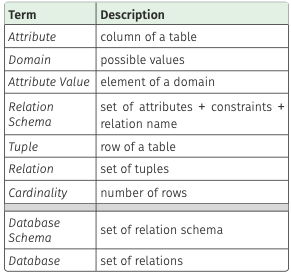
\includegraphics[width=1.0\linewidth]{1_relational_model.png}
      \columnbreak
        \\ \underline{Relational Schema:} Defines a relation, specifies attributes (columns), data constraints, name 
        \begin{itemize}
          \item $R(A_1, A_2, \dots A_3)$: relation schema with name $R$ and $n$ attributes $A_1, A_2, \dots, A_n$
          \item Eg. \verb|Employees(id:INT,| \verb|name:TEXT, dob:TEXT)|
        \end{itemize}
    \end{multicols}
    \underline{Domain:} Set of atomic values, including NULL
    \begin{itemize}
      \item $dom(A_i)$ = set of possible values for $A_i$
      \item $\forall$ value $v$ of attribute $A_i$, $v \in \{dom(A_i \cup \{null\})\}$
    \end{itemize}

    \subsection{Keys}
    \begin{itemize}
      \item \textbf{Superkey:} Subset of attributes that UNIQUELY IDENTIFIES  a tuple in a relation
      \item \textbf{Key:} Superkey that is also MINIMAL (No proper subset of key is a superkey)
      \item \underline{Properties of Superkeys \& Keys:}
      \begin{enumerate}
        \item If (A,B,C) is DEFINITELY superkey $\rightarrow$ (A,B,C,D) is superkey
        \item If (A,B,C) is DEFINITELY key $\rightarrow$ (A,B,C) is superkey
        \item If (A,B) is DEFINITELY superkey $\rightarrow$ (A,B,C) is NOT a key
        \item If (A,B) is DEFINITELY key $\rightarrow$ possible (B,C,D) is also key
        \item Every relation has $\geq$ 1 superkey
      \end{enumerate}
      \item \textbf{Candidate Key:} Set of all keys of a given relation
      \item \textbf{Primary Key:} A selected candidate key (attributes CANNOT be NULL, is underlined in schema notation)
      \item \textbf{Foreign Key:} Subset of attributes of relation $R_1$ that refers to Primary Key of relation $R_2$
      \begin{itemize}
        \item $R_1$ is referencing relation, $R_2$ is referenced relation
        \item $R.sid \rightarrow S.id$: $R.sid$ is a FK referencing PK $id$ in $S$
        \item FK in $R_1$ must appear as PK in $R_2$ OR be NULL/tuple containing at least 1 NULL value
        \item A referencing relation can be a referenced relation for different foreign key $\vert$ Referencing relation \& referenced relation can be same relation
      \end{itemize}
    \end{itemize}

    \section{SQL}
    \subsection{Three-valued Logic / Handing NULLs}
    \begin{itemize}
      \item \textbf{Logical Operations}
      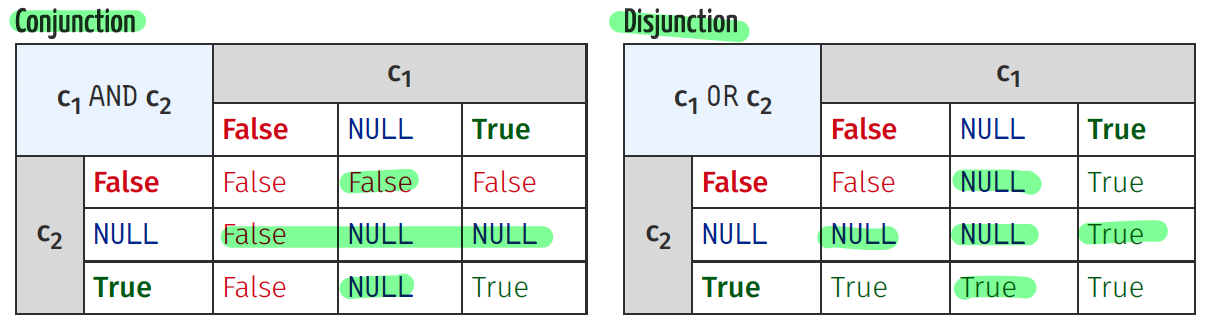
\includegraphics[width=1.0\linewidth]{2_three_valued_logic.png}
      \begin{itemize}
        \item \textbf{Implication:} $C_1 \rightarrow C_2$ == $(\sim C_1) \vee C_2$
        \item $\sim NULL$ == $NULL$
      \end{itemize}
      \item \textbf{Relational Operations:} Any relational operations with $NULL$ produced $NULL$ values (Eg. $\leq$, $=$, $!=$)
      \item \textbf{Arithmetic Operations:} Any arithmetic operations with $NULL$ produces $NULL$ values
      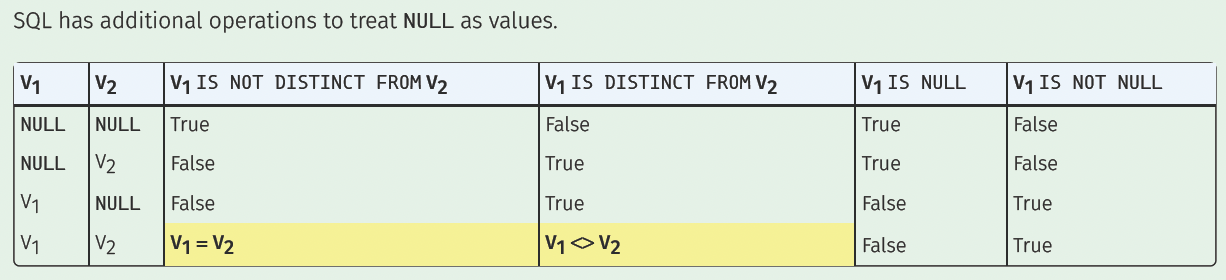
\includegraphics[width=1.0\linewidth]{3_nulls.png}
      \item \textbf{IS NULL vs = NULL (in WHERE clause):} IS NULL will select NULL values $\vert$ = NULL will not select any NULL values (NULL = NULL $\rightarrow$ NULL, nothing will be selected by Principle of Acceptance)
      \item \textbf{DISTINCT keyword (in SELECT clause):} DISTINCT checks for distinct rows using IS DISTINCT FROM (Duplicate NULL values are removed)
      \item \textbf{Empty \& NULL Semantics in Aggregate functions}
      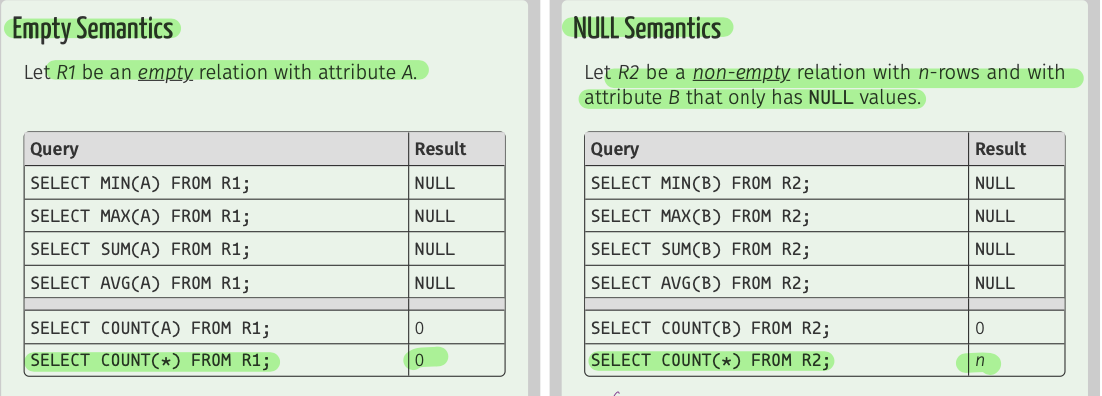
\includegraphics[width=1.0\linewidth]{4_empty_null_semantics.png}

      \subsection{Integrity Constraints}
      \begin{itemize}
        \item \textbf{Principle of Rejection:} Integrity Constraints follow POR (Rejects insertion if condition evaluates to FALSE, Insertion is still done if condition is NULL) 
      \end{itemize}
      \begin{enumerate}
        \item \underline{NOT NULL:} Rejects insertion if value at specified column is NULL (Condition: IS NOT NULL)
        \item \underline{UNIQUE:} Rejects insertion if there are other rows where values are equal (Condition: $x.A_i <> y.A_i$) $\vert$ Can have multiple NULL values since NULL $<>$ NULL == NULL
        \item \underline{Primary Key:} Equivalent to UNIQUE \& NOT NULL $\vert$ If one of the attributes is NULL, entire tuple is rejected
        \item \underline{Foreign Key:} Rejects insertion if tuple does not exist in referenced relation AND is NOT NULL
        \begin{itemize}
          \item NO ACTION: Rejects delete/update if it violates constraints
          \item CASCADE: Propagates delete/update to referencing tuples
          \item SET DEFAULT: Updates FK of referencing tuples to default value
          \item SET NULL: Updates FK of referencing tuples to NULL value
        \end{itemize}
        \item \underline{CHECK:} Rejects insertion if condition is FALSE
      \end{enumerate}
    \end{itemize}

    \subsection{Deferrable Constraints}
    \begin{itemize}
      \item \textbf{Default Behaviour:} Constraints are checked immediately at end of SQL statement $\rightarrow$ Violation of 1 of the statements will cause whole transaction to roll black
      \item \textbf{Benefit:} Allow cyclic FK constraints
    \end{itemize}
    \begin{enumerate}
      \item \underline{NOT DEFERRABLE:} Constraint checks are not deferred at all
      \item \underline{DEFERRABLE INITIALLY DEFERRED:} Constraint checks are deferred right at the start
      \item \underline{DEFERRABLE INITIALLY IMMEDIATE:} Constraint checks are not deferred until DEFERRED keyword in transaction (Defer constraints on demand)
    \end{enumerate}

    \subsection{Set Operations}
    \begin{itemize}
      \item \textbf{Union Compatible:} 2 relations are union-compatible if (1): Both have same \# of attributes, (2): Corresponding attributes have same or compatible domains (Similar to function signatures where number, order \& type matters)
      \item \textbf{Remove Duplicates:} \verb |UNION, INTERSECT, EXCEPT|
      \item \textbf{Keep Duplicates:} \verb|UNION ALL, INTERSECT ALL, EXCEPT ALL| (Treats each element as distinct element)
    \end{itemize}
    
    \subsection{Subqueries}
    \begin{itemize}
      \item Appears in \verb|SELECT, FROM, WHERE|
      \item \textbf{IN/NOT IN}: Subquery must return exactly 1 column $\vert$ If expression matches any subquery row $\rightarrow$ IN returns TRUE, NOT IN returns FALSE $\vert$ If subquery evaluates to empty table $\rightarrow$ IN returns TRUE, NOT IN returns FALSE
      \item \textbf{EXISTS/NOT EXISTS}: Subquery may return any \# of columns $\vert$ If expression matches any subquery row $\rightarrow$ EXISTS returns TRUE, NOT EXISTS returns FALSE $\vert$ If subquery evaluates to empty table, EXISTS returns FALSE, NOT EXISTS returns TRUE $\vert$ Only emptiness of subquery matters (Use \verb|SELECT 1|)
      \item \textbf{ANY/ALL}: Subquery must return exactly 1 column $\vert$ ANY returns TRUE if comparison is true to $\geq$ 1 row, ALL returns TRUE if comparison is true to all rows  $\vert$ If subquery evaluates to empty table, ANY returns FALSE, ALL returns TRUE
    \end{itemize}

    \subsection{Conceptual Evaluation}
    \begin{enumerate}
      \item \textbf{FROM}: Compute cross product/JOINs of all Tables in FROM clause
      \item \textbf{WHERE}: Keep tuples that evaluates to TRUE on the WHERE condition (WHERE follows Principle of Acceptance $\vert$ Cannot use aggregate directly in WHERE, but can have sub-query which contains aggregate in WHERE)
      \item \textbf{GROUP BY}: Partition table into groups w.r.t grouping attributes (Application of aggregate functions are over each group $\rightarrow$ 1 result tuple per group)
      \item \textbf{HAVING}: Keep groups that evaluates to TRUE on the HAVING condition (Conditions typically involve aggregates)
      \item \textbf{SELECT}: Remove all attributes not specified in SELECT clause (Remove duplicates if DISTINCT)
      \item \textbf{ORDER BY}: Sort tables based on specified attributes
      \item \textbf{LIMIT/OFFSET}: Keep tuples based on their order in table
    \end{enumerate}
    \textbf{Restriction to SELECT/HAVING clauses upon GROUP BY}: If column $A_i$ of table R appears in SELECT/HAVING clause, $A_i$ must appear in GROUP BY clause OR $A_i$ appear as input of aggregate function in SELECT/HAVING clause OR PK of R appears in GROUP BY clause

    \subsection{Special Functions}
    \begin{enumerate}
      \item \textbf{Patter Matching:} \_ matches any single character, \% matches any sequence of 0 or more characters (eg. \verb|WHERE pizza LIKE 'Ma%a'|)
      \item \textbf{COALESCE}: Returns 1st non-NULL value in list of input arguments, returns NULL if all values in list are NULL
      \item \textbf{NULLIF:} Returns NULL if $value_1$ = $value_2$, otherwise return $value_1$
    \end{enumerate}

    \subsection{Universality}
    \begin{itemize}
      \begin{multicols}{2}
        \item \textbf{Double Negation Method:} $\forall x: Exist(x)$ == $\sim\exists x: \sim Exist(x)$
        \item Eg. Restaurants that sells ALL pizzas liked by 'Homer' == There does not exist pizza that 'Homer' likes \& not sold by the restaurant
        \columnbreak
        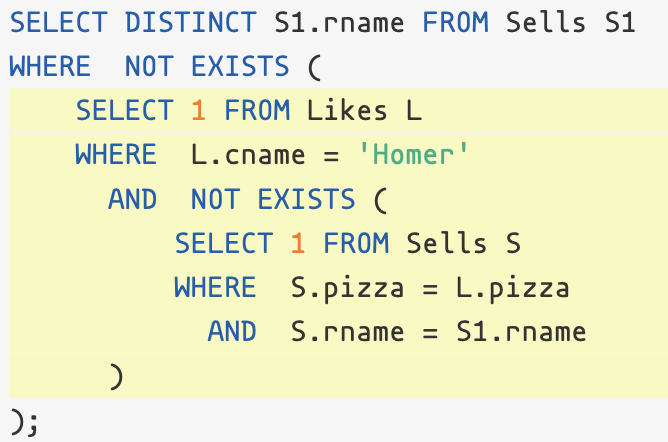
\includegraphics[width=1.0\linewidth]{5_double_negation.png}
      \end{multicols}
      \item \textbf{Cardinality Method:} \\ $S \subseteq R$ $\rightarrow$ $\mid R \cup S \mid = \mid R \mid$, $\mid R \cap S \mid = \mid S \mid$ \\ $R \equiv S$ $\rightarrow$ $\mid R \cup S \mid = \mid R \cap S \mid$
    \end{itemize}

    \subsection{Recursive CTE}
    \underline{Eg.} Find all MRT stations that can be reached from NS1 in at most 3 stops \\
      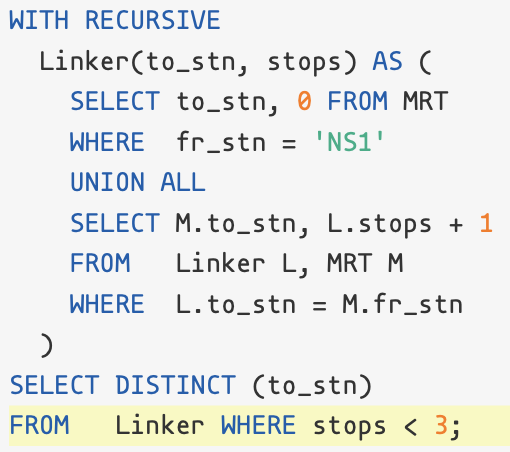
\includegraphics[width=0.45\linewidth]{6_recursive_cte_eg.png}

    \section{Entity Relationship Model}
    \subsection{Entity Relationship}
    \begin{itemize}
      \item \textbf{Entities:} Nouns (Rectangles), \textbf{Relationships:} Verbs (Diamonds)
      \item \textbf{Attributes:} Describe info about entities \& relationships
      \begin{enumerate}
        \item \underline{Key attribute:} Uniquely identifies each Entity
        \item \underline{Composite attribute:} Composed of multiple other attributes
        \item \underline{Multi-valued attributes:} 1 or more values for a given Entity
        \item \underline{Derived attributes:} Derived from other attributes
        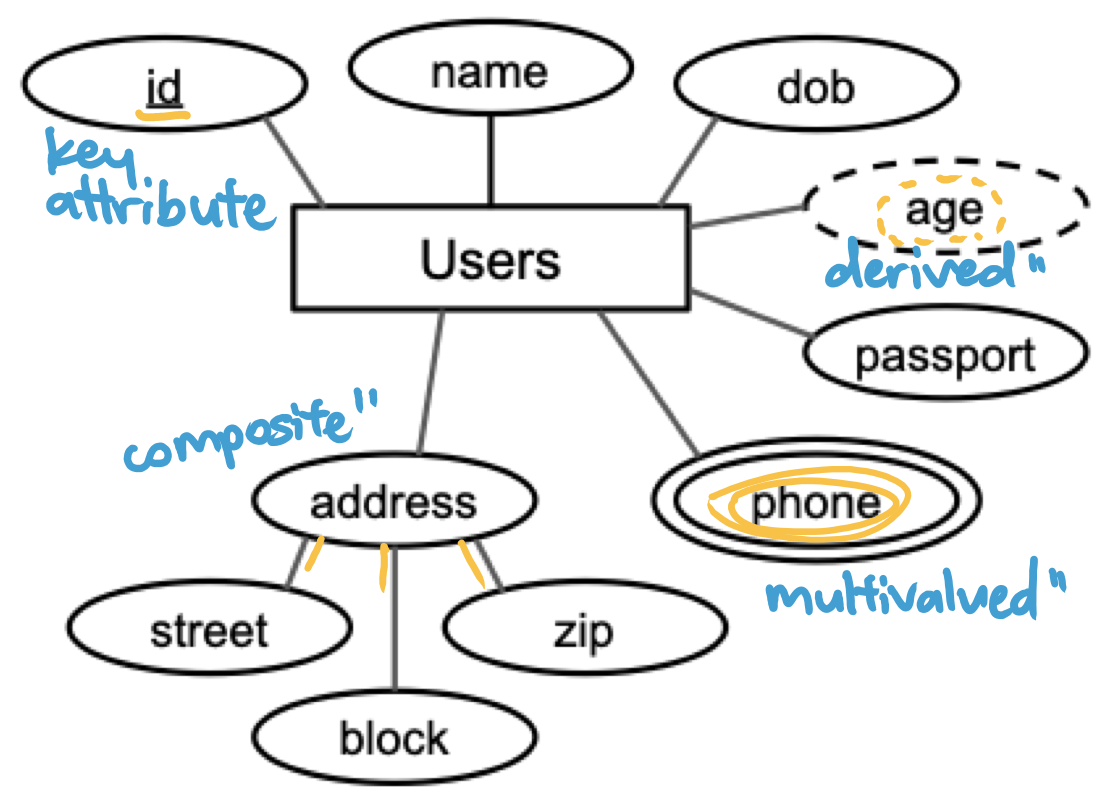
\includegraphics[width=0.55\linewidth]{7_attribute_subtypes.png}
      \end{enumerate}
      \item \textbf{Degrees of Relationship Sets:} \# of entity sets (can be non-unique) involved in relationship set
    \end{itemize}

    \subsection{Relationship Constraints}
    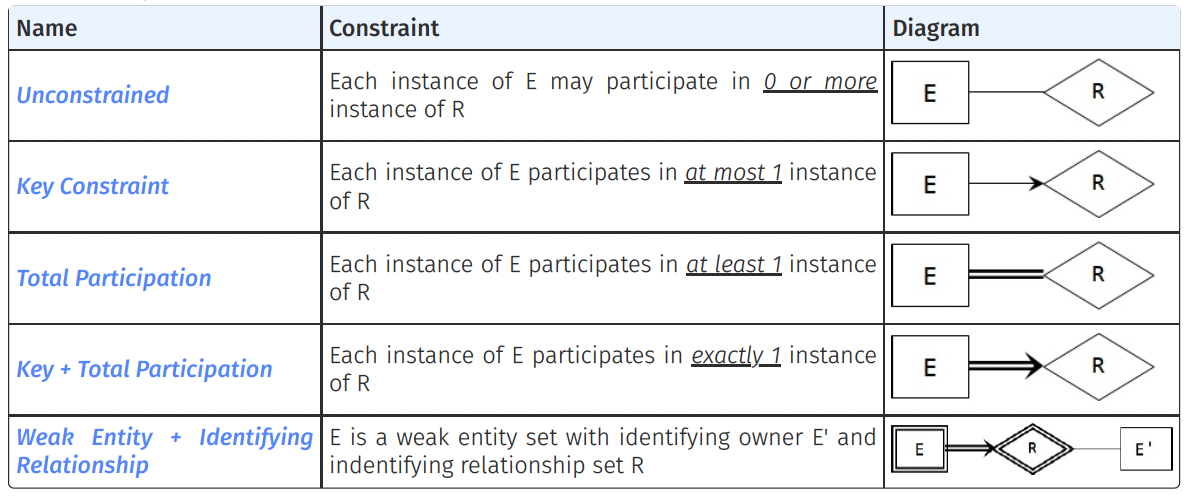
\includegraphics[width=1.0\linewidth]{8_summary_relationship_constraints.png}
    \textbf{Weak Entity Set:} An entity set that does not have its own key (Has partial key that cannot uniquely identify an entity) $\rightarrow$ Needs help of key from \underline{Owning Entity Set} to uniquely identify an entity
    
    \subsection{Relational Mapping (ER to Schema)}
    \textbf{Entity Set}
    \begin{enumerate}
      \item \underline{Name} of entity set $\rightarrow$ Name of table
      \item \underline{Attribute} of entity set $\rightarrow$ Column of table
      \item \underline{Key attribute} of entity set $\rightarrow$ PK of table
      \item \underline{Derived attribute} of entity set $\rightarrow$ Should not appear in table
      \item \underline{Composite attribute} of entity set $\rightarrow$ Converted into decomposed attributes in table
      \item \underline{Multi-valued attribute} of entity set $\rightarrow$ Converted into seq. of single-valued attributes OR Create another table with FK constraint
    \end{enumerate}
    \textbf{Relationship Set}
    \begin{enumerate}
      \item \underline{Many-to-Many Relationship:} Relationship Set Schema should have its PK including PKs of both entities
      \item \underline{Many-to-One Relationship:} 
      \begin{itemize}
        \item \textit{Separate Tables strategy:} Relationship Set Schema should have PK of One-Set as its PK to enforce upper bound of 1 \&  PK of Many-Set in Relationship Set should be NOT NULL to prevent redundant info
        \item \textit{Combined Tables strategy:} Combine Relationship Set with One-Set, PK of merged set is PK of One-Set, PK of Many-Set in merged set can be NULL
      \end{itemize}
      \item \underline{One-to-One Relationship:}
      \begin{itemize}
        \item \textit{No Relationship Set strategy:} PK of each entity set is a UNIQUE FK in other set
        \item \textit{3 Table strategy:} Relationship Set Schema has its PK as PK of 1 of the entity set, other entity set's PK appears in Relationship Set Schema as a UNIQUE, NOT NULL FK (candidate key)
      \end{itemize}
      \item \underline{Key + Total Relationship:} Combine Relationship Set with KeyTotal-Set, PK of merged set is PK of KeyTotal-Set, PK of Many-Set in Relationship Set must be NOT NULL
      \item \underline{Weak Entity Set Relationship:} Combine Relationship Set with Weak Entity Set, PK of merged set is combination of Owning Entity Set's PK \& Weak Entity Set's PK, PK of Owning Entity Set appears as FK in merged set with ON DELETE/UPDATE CASCADE 
    \end{enumerate}
    \textbf{NOTE:} Total Participation Constraint in ER model cannot be enforced by schema

    \subsection{ISA Hierarchy}
    \begin{itemize}
      \item Subclass must be uniquely identified by same key attributes of superclass (subclass keys should not be shown in ER diagram)
      \item Subclass may have additional attribute \& involved in additional relationship
      \item \textbf{Schema Syntax:} Subclass has Superclass's PK as its PK \& FK (along with ON DELETE CASCADE)
      \begin{multicols}{2}
        \noindent
        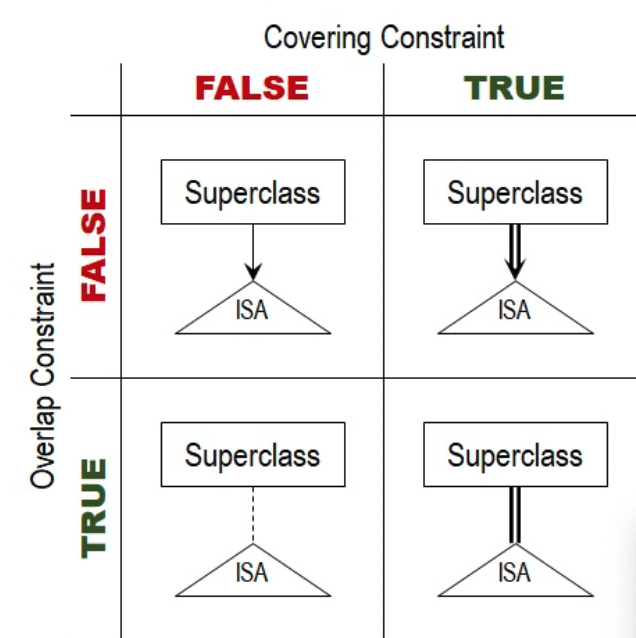
\includegraphics[width=0.9\linewidth]{9_ISA.png}
        \columnbreak
        \begin{enumerate}
          \item Overlap Constraint (Upper bound): Can a superclass belong to multiple subclasses? FALSE sets Upper bound = 1 (Key constraint)
          \item Covering Constraint (Lower bound): Must a superclass belong to $\geq$ 1 subclass? TRUE sets Lower bound = 1 (Total Participation constraint)
        \end{enumerate}
      \end{multicols}
    \end{itemize}

    \subsection{Aggregation}
    \begin{itemize}
      \item Aggregate is a relationship set \& entity set
      \item Key attributes are formed from relationship set
    \end{itemize}
    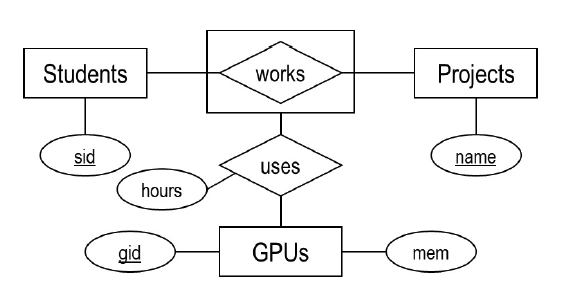
\includegraphics[width=0.55\linewidth]{10_aggregate_diagram.png}
    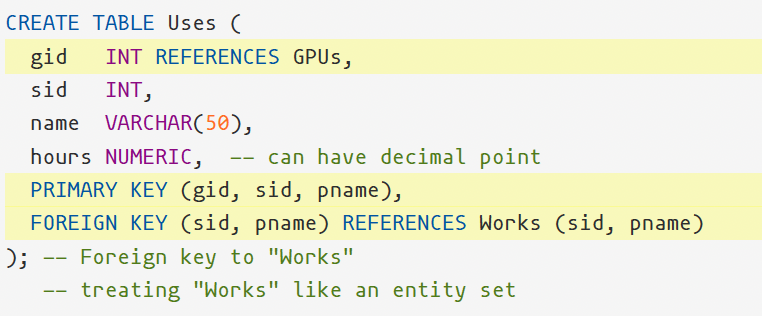
\includegraphics[width=0.75\linewidth]{11_aggregate_schema.png}
    \begin{multicols}{2}
      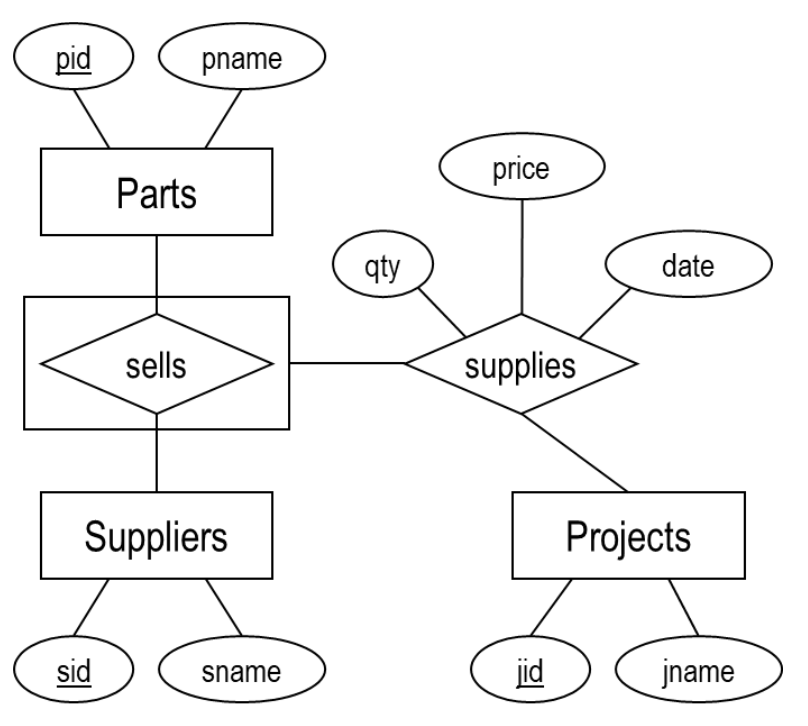
\includegraphics[width=0.8\linewidth]{12_aggregate_example.png}
      \begin{itemize}
        \item Supplier can sell Part without being used by a Project
        \item Aggregate's relationship set depicts necessary relationship btw. 2 entity sets
        \item Aggregate's entity set depicts optional relationship
      \end{itemize}
    \end{multicols}

    \section{Relational Algebra}
    \subsection{Algebra}
    \textbf{Closure:} A set of values is closed under the set of operators if any combination of the operators produces only values in the given set (Relations are closed under Relational Algebra)
    
    \subsection{Unary Operators}
    \textbf{Selection Operator ($\sigma$)}
    \begin{itemize}
      \item $\sigma_{[c]}(R)$ : Selects all tuples from relation $R$ (ROWS) that satisfies the selection condition $c$ based on Principle of Acceptance
      \item $c$ is a condition that returns a boolean (potentially NULL), $c$ must specify only attributes in $R$
      \item \underline{Precedence:} $(), op, \neg , \wedge , \vee$
      \item Can be mapped to \verb|WHERE| clause of SQL
      \item \underline{Properties:} Result have same schema as input relation $\vert$ \# of rows are often smaller
    \end{itemize}
    \textbf{Projection Operator ($\pi$)}
    \begin{itemize}
      \item $\pi_{[l]}(R)$ : Keeps only columns specified in ordered list $l$ and in same order 
      \item $l$ must specify only attributes in $R$, No operations \& duplicates in projection operator (eg. $\pi_{[A_1 + A_2]}(R)$, $\pi_{[A_1, A_1]}(R)$)
      \item $\pi_{[A_1, A_2]}(R) \neq \pi_{[A_2, A_1]}(R)$ (Order matters!!)
      \item Can be mapped to \verb|SELECT| clause in SQL
      \item \underline{Properties:} Resulting schema is as specified by $l$ without relation name $\vert$ \# of rows may be smaller (Relation is defined as set of tuples $\rightarrow$ Duplicate rows will be removed)
    \end{itemize}
    \textbf{Renaming Operator ($\rho$)}
    \begin{itemize}
      \item $\rho_{[r]}(R)$ : Renames all attributes mentioned in $r$ s.t. for each renaming $B_i \leftarrow A_i$, $A_i$ is renamed to $B_i$
      \item Can be mapped to \verb|AS| keyword in \verb|SELECT| in SQL
      \item \underline{Properties:} Resulting schema is old schema renamed by $r$ $\vert$ Order of column is unchanged (except for renaming) $\vert$ \# of rows remains the same
    \end{itemize}

    \subsection{Binary Operators}
    \textbf{SET Operators}
    \begin{itemize}
      \item $R \cap S$, $R \cup S$, $R - S$ (Relations must be union-compatible)
    \end{itemize}
    \textbf{PRODUCT Operators}
    \begin{itemize}
      \item $R \times S$ : Cross product of 2 relations is a relation formed by combining all pairs of tuples from 2 input relations
      \item Can be mapped to \verb|FROM| keyword in SQL
      \item \underline{Optimisation:} Cross product can be optimised by \verb|JOIN| operators, which combines cross product, selection \& projection (Avoids generating all $\vert R \times S \vert$ intermediate tuples)
    \end{itemize}
    \textbf{INNER JOIN Operators}
    \begin{enumerate}
      \item \textbf{$\theta$ Join:} $R \Join_{[\theta]}S$ = $\sigma_{[\theta]}(R \times S)$ (Cross product followed by selection)
      \item \textbf{Equi Join}: $R \Join_{[=]}S$ = Special $\theta$ Join where the only relational operator used is equality (All equi join is a $\theta$ join but not all $\theta$ join are equi join)
      \item \textbf{Natural Join:} $R \Join S$ = $\pi_{[l]} (\sigma_{[\theta]}(R \times S))$
      \begin{itemize}
        \item $l$ = $(Attr(R) \cap Attr(S)) + (Attr(R) - Attr(S)) + (Attr(S) - Attr(R))$ (Order matters, where common attributes are listed, then R's attributes, followed by S's attributes)
        \item $\theta$ = $\forall \in (Attr(R) \cap Attr(S)): R.A_i = S.A_i$ (All common attributes are equal)
      \end{itemize}
    \end{enumerate}
    \textbf{OUTER JOIN Operators}
    \begin{enumerate}
      \item \textbf{Semi Join:} $R \ltimes_{[\theta]}S$ = $\pi_{[Attr(R)]}(R \Join_{[\theta]}S)$ (Used to find non-dangling tuple)
      \\ NOTE: Semi Join projects R's attributes only, while normal Joins will project R and S's attributes
      \item \textbf{Dangles:} $dangle(R \Join_{[\theta]}S)$ = $R - R \ltimes_{[\theta]}S$
      \item \textbf{Left Outer Join:} $R_1 \leftouterjoin_{[c]}R_2$ = Inner Join $\cup$ Left Dangling Tuple = $R_1 \Join_{[c]} R_2 \cup (dangle(R_1 \Join_{[\theta]}R_2) \times (null(R_2))$
      \item \textbf{Right Outer Join:} $R_1 \rightouterjoin_{[c]}R_2$ = Inner Join $\cup$ Right Dangling Tuple = $R_1 \Join_{[c]} R_2 \cup ((null(R_1) \times dangle(R_2 \Join_{[\theta]}R_1))$
      \item \textbf{Full Outer Join:} $R_1 \fullouterjoin_{[c]}R_2$ = Inner Join $\cup$ Left Dangling Tuple $\cup$ Right Dangling Tuple = $R_1 \Join_{[c]} R_2 \cup (dangle(R_1 \Join_{[\theta]}R_2) \times (null(R_2)) \cup ((null(R_1) \times dangle(R_2 \Join_{[\theta]}R_1))$
    \end{enumerate}

    \subsection{Complex Expressions}
    \textbf{Equivalence VS Isomorphic}
    \begin{itemize}
      \item \underline{Equivalence ($\equiv$):} 2 relational algebra expressions are equivalent if both produces same result with same column order, possibly different row order
      \item \underline{Isomorphic ($\cong$):} 2 relational algebra expressions are isomorphic if both produces same result with possibly different column order, possibly different row order
    \end{itemize}
    \textbf{Special Properties}
    \begin{enumerate}
      \item $\sigma_{[\theta_1]}(\sigma_{[\theta_2]}(R)) \equiv \sigma_{[\theta_2]}(\sigma_{[\theta_1]}(R)) \equiv \sigma_{[\theta_1 \wedge \theta_2]}(R)$
      \item $\pi_{[l_1]}(\pi_{[l_2]}(R)) \nequiv \pi_{l_1}(R)$ unless $l_1 \subseteq l_2$
      \item $R \times S \cong S \times R$, $R \Join S \cong S \Join R$, $R \Join (S \Join T) \cong (R \Join S) \Join T$ (Different column order)
      \item $R \times (S \times T) \equiv (R \times S) \times T$ (Associative)
      \item $\pi_{[l]}(\sigma_{[\theta]}(R)) \nequiv \sigma_{[\theta]}(\pi_{[l]}(R))$ (Unless $\theta$ uses only attributes in $l$)
      \item $\sigma_{[\theta]}(R \times S) \nequiv \sigma_{[\theta]}(R) \times S$ (Unless $\theta$ uses only Attr($R$))
    \end{enumerate}

    \section{Functions \& Procedures}
    \subsection{Functions}
    \begin{itemize}
      \item Returns some values/tuples
      \item \textbf{Returns output of an atomic data type:}
      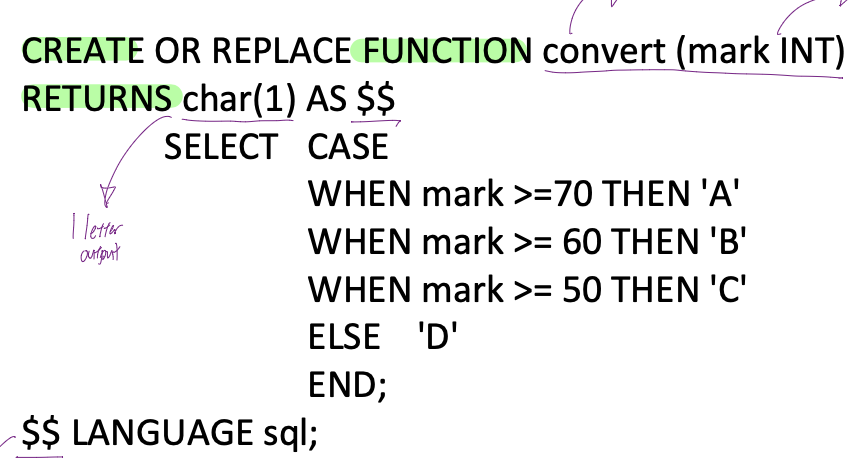
\includegraphics[width=0.55\linewidth]{13_func_atomic.png} \\
      \underline{Example Query:} \verb|SELECT Name, convert(Mark) FROM Scores;|
      \item \textbf{Returns 1 EXISTING tuple:}
      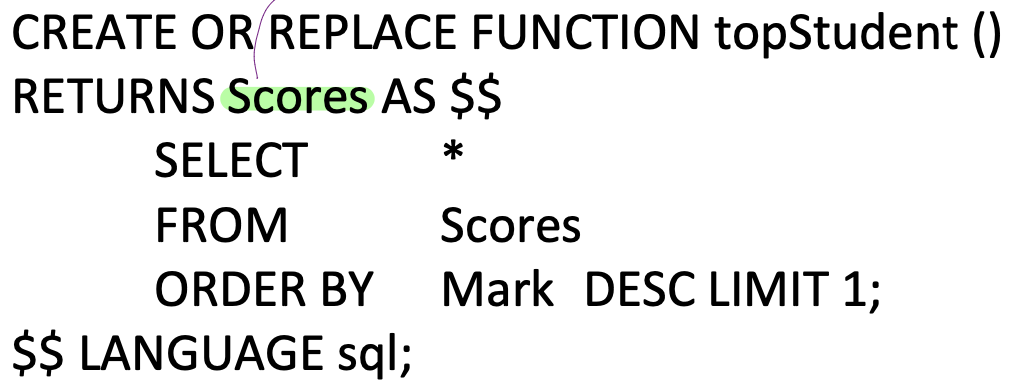
\includegraphics[width=0.55\linewidth]{14_func_existing.png} \\
      \underline{Example Query:} \verb|SELECT topStudent();|
      \item \textbf{Returns EXISTING SET of tuples:}
      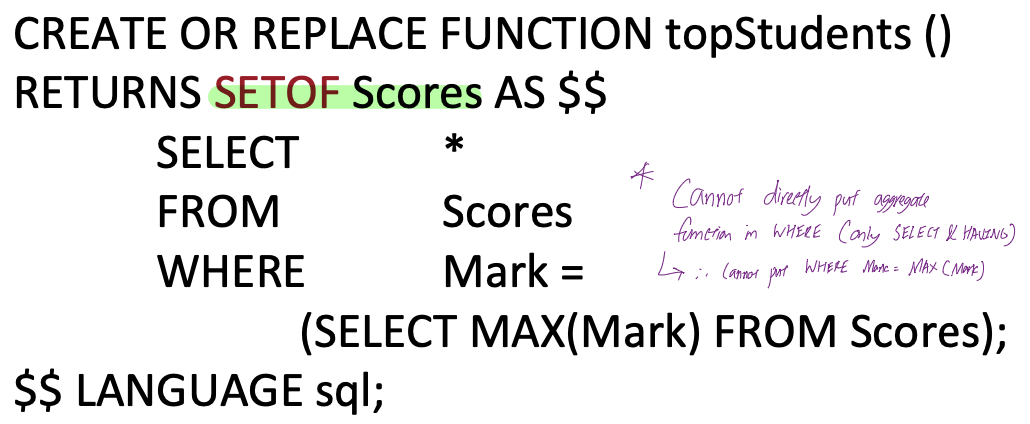
\includegraphics[width=0.55\linewidth]{15_func_existing_set.png} \\
      \underline{Example Query:} \verb|SELECT * FROM topStudents();|
      \item \textbf{Returns 1 NEW tuple (Note parameters):} \\
      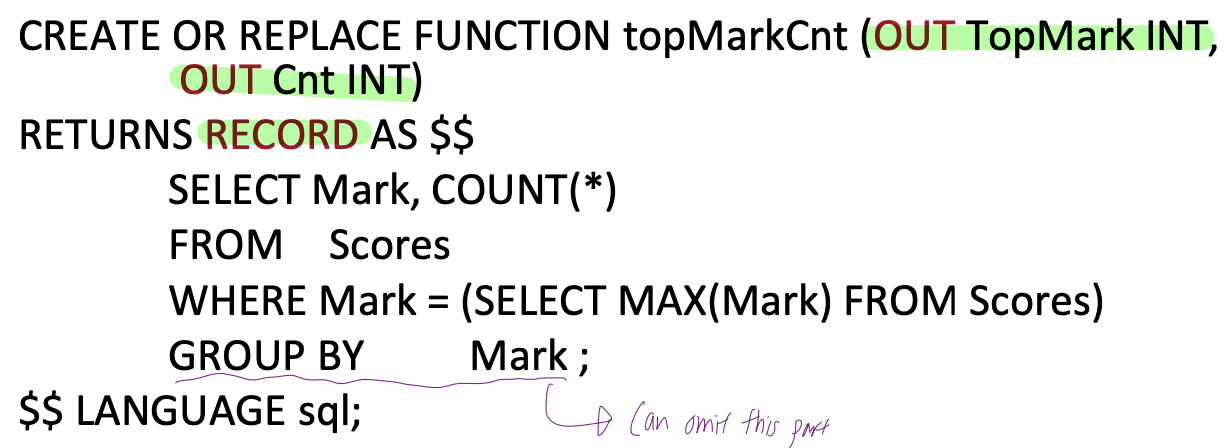
\includegraphics[width=0.65\linewidth]{16_func_new.png} \\
      \underline{Example Query:} \verb|SELECT topMarkCnt();|
      \item \textbf{Returns NEW SET of tuples (Note parameters):}
      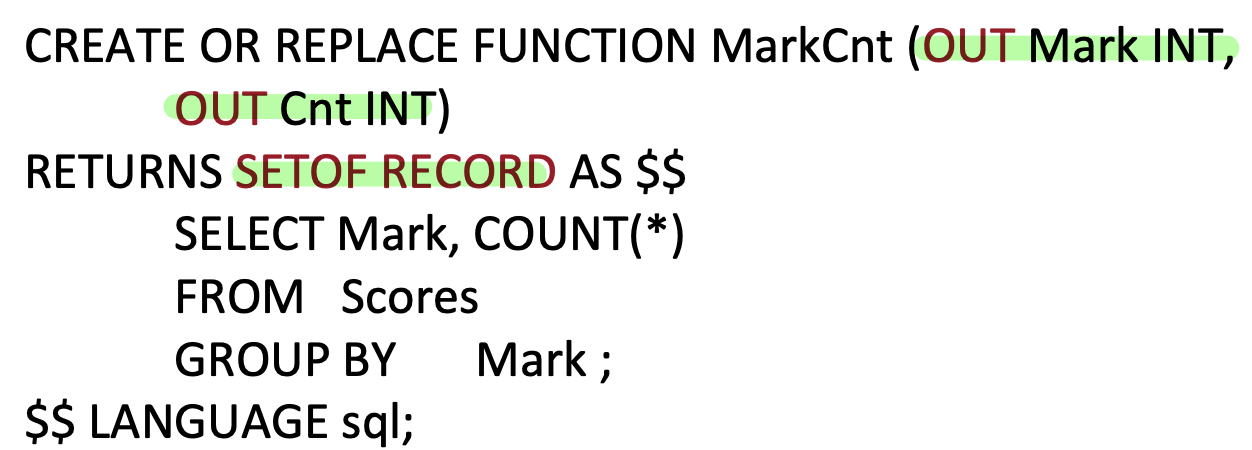
\includegraphics[width=0.55\linewidth]{17_func_new_set.png} \\
      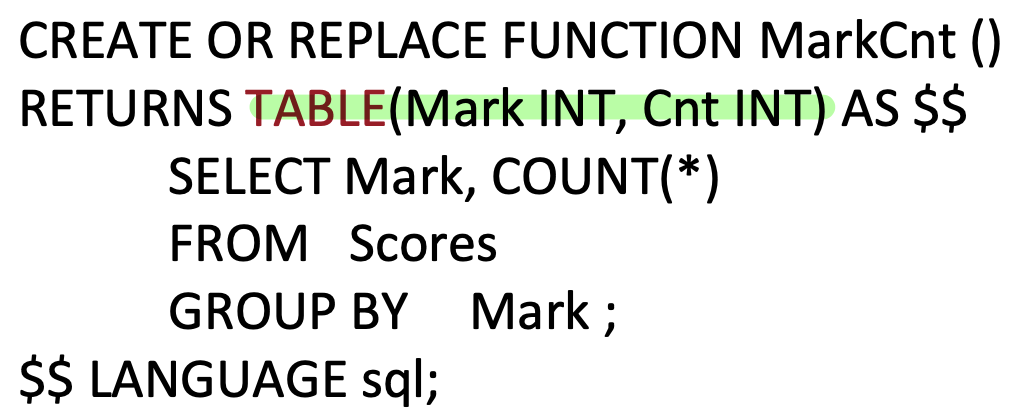
\includegraphics[width=0.55\linewidth]{18_func_new_table.png} \\
      \underline{Example Query:} \verb|SELECT MarkCnt();|
    \end{itemize}

    \subsection{Procedures}
    \begin{itemize}
      \item Do not return value/tuple
      \item \underline{Syntax}: \verb|CREATE OR REPLACE PROCEDURE...|
    \end{itemize}
    \subsection{Control Structures:}
    \begin{enumerate}
      \item \verb|IF ... THEN ... ELSE ... END IF|
      \item \verb|LOOP ... END LOOP|
      \item \verb|EXIT ... WHEN ...|
      \item \verb|WHILE ... LOOP ... END LOOP|
      \item \verb|FOR ... IN ... LOOP ... END LOOP|
    \end{enumerate}

    \subsection{Variables:}
    \begin{itemize}
      \item Variables are declared in \verb|DECLARE| section, Actual function is in \verb|BEGIN ... END| section
      \item Values are selected into variables (\verb|SELECT COUNT(*) INTO| \verb|overlap_count|) OR assigned directly (\verb|temp_val := val1|)
    \end{itemize}

    \subsection{Cursor:}
    \begin{itemize}
      \item Cursor enables us to access each individual row selected by a \verb|SELECT| statement (DECLARE $\rightarrow$ OPEN $\rightarrow$ FETCH $\rightarrow$ CLOSE)
      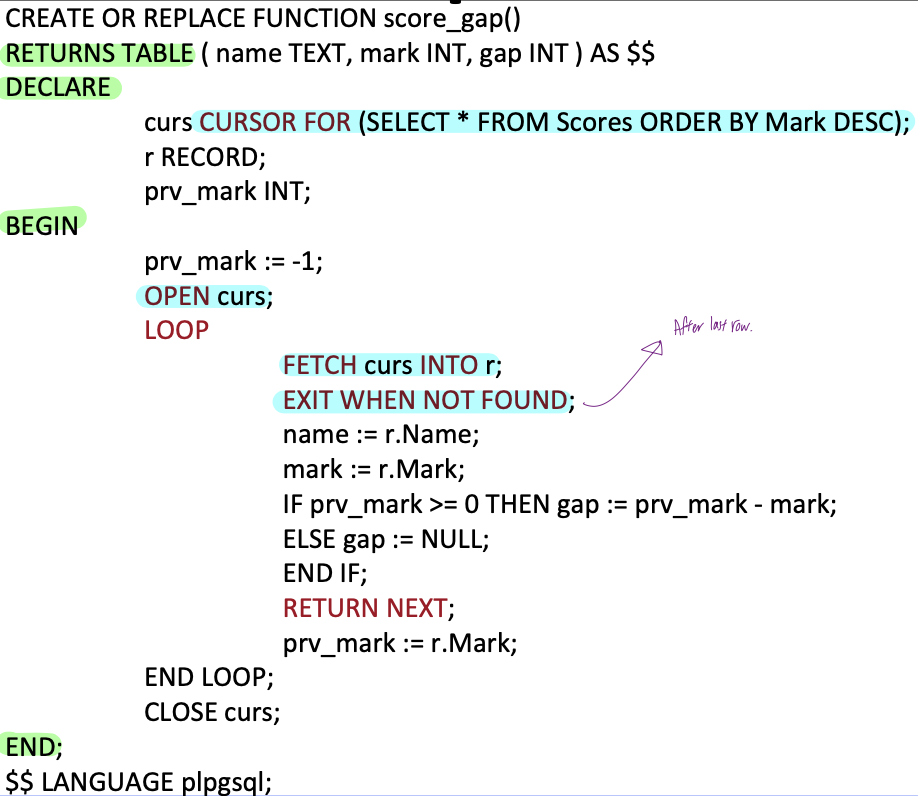
\includegraphics[width=0.7\linewidth]{19_cursor.png}
      \item \verb|OPEN|: SQL statement for cursor is executed \& cursor points to beginning of result
      \item \verb|FETCH|: Next tuple from cursor is read \& put into \verb|r| $\rightarrow$ No tuple, terminate loop
      \item \verb|RETURN NEXT|: Inserts a tuple to output of function
      \item \verb|CLOSE|: Releases resources allocated to cursor
      \item \underline{Cursor Movement:} \verb|FETCH PRIOR FROM cur INTO r|, \verb|FETCH| \verb|FIRST FROM cur INTO r|, \verb|FETCH LAST FROM cur INTO r|, \verb|FETCH ABSOLUTE x FROM cur INTO r| (fetch x\textsuperscript{th} tuple)
    \end{itemize}
  \end{multicols*}
\end{document}
